\begin{figure}[ht!]
  \centering
  \begin{tikzpicture}
    \begin{groupplot}[disabledatascaling,group style={vertical sep=0cm, group size=1 by 2}, width=\textwidth, height=8.5cm, xlabel=Wellenlänge $\lambda$ in \si{\micro\metre},xmin=.5, xmax=3.5, legend cell align={left}, ymin=-.07, ymax=1.395]
      \nextgroupplot[ylabel={Energiedichte in a.u.}, y label style={xshift=-3cm, yshift=0cm}, xlabel={}, xticklabels]
      \addplot[blue, thick] table[x index=0,y index=1, x expr=0.001*\thisrowno{0}]{Daten/Kalibrierung_Glasprisma_Wolframlampe2V_3_6Grad_500-3200nm_mitMarkern2_Spalt_500mu.txt};
      \addplot[domain=.5:3.5,thick, orange, no marks, samples=200]{1291/(x^5*(exp(14388/(x*1867))))};
      \draw[thick, <-] (1.255,0.788) -- +(0,0.2)node[above]{\SI{1.255}{\micro\metre}};
      \draw[thick, <-] (1.412,0.29) -- +(0,-0.2)node[below]{\SI{1.412}{\micro\metre}};
      \draw[thick, <-] (1.552,1) -- +(0,0.2)node[above]{\SI{1.552}{\micro\metre}};
      \draw[thick, <-] (1.886,0.587) -- +(0,-0.2)node[below]{\SI{1.886}{\micro\metre}};
      \draw[thick, <-] (1.932,0.569) -- +(0,0.35)node[above]{\SI{1.932}{\micro\metre}};
      \draw[thick, <-] (2.254,-0.03) -- +(0,0.45)node[above]{\SI{2.254}{\micro\metre}};
      \legend{Messkurve \SI{2}{\volt}, Theoretische Kurve (\SI{1867}{\kelvin})};
      \nextgroupplot[]
      \addplot[blue, thick] table[x index=0,y index=1, x expr=0.001*\thisrowno{0}]{Daten/Kalibrierung_Glasprisma_Wolframlampe5V_3_6Grad_500-3200nm_mitMarkern2_Spalt_500mu.txt};
      \addplot[domain=.5:3.5,thick, orange, no marks, samples=200]{405/(x^5*(exp(14388/(x*2362))))};
      \draw[thick, <-] (.832,0.1556) -- +(0,0.2)node[above, fill=white, fill opacity=0.4, text opacity=1]{\SI{.832}{\micro\metre}};
      \draw[thick, <-] (1.227,1) -- +(0,0.2)node[above]{\SI{1.227}{\micro\metre}};
      \draw[thick, <-] (1.269,0.967) -- +(0,-0.2)node[below, fill=white, fill opacity=0.4, text opacity=1]{\SI{1.269}{\micro\metre}};
      \draw[thick, <-] (1.408,0.358) -- +(0,-0.2)node[below]{\SI{1.408}{\micro\metre}};
      \draw[thick, <-] (1.888,0.433) -- +(0,-0.2)node[below]{\SI{1.888}{\micro\metre}};
      \draw[thick, <-] (1.930,0.414) -- +(0,0.3)node[above]{\SI{1.930}{\micro\metre}};
      \draw[thick, <-] (2.248,0) -- +(0,0.3)node[above]{\SI{2.248}{\micro\metre}};
      \legend{Messkurve \SI{5}{\volt}, Theoretische Kurve (\SI{2362}{\kelvin})};
    \end{groupplot}
  \end{tikzpicture}
  \caption{Spektrale Energiedichte einer Wolframdampflampe bei zwei unterschiedlichen Betriebsspannungen. An das Wellenlängenmaximum wurde jeweils eine \textsc{Planck}-Kurve zum Vergleich angefittet.}
  \label{fig:Wolframlampe}
\end{figure}

% \begin{figure}[htp]
%   \centering
%   \begin{subfigure}{0.9\textwidth}
%     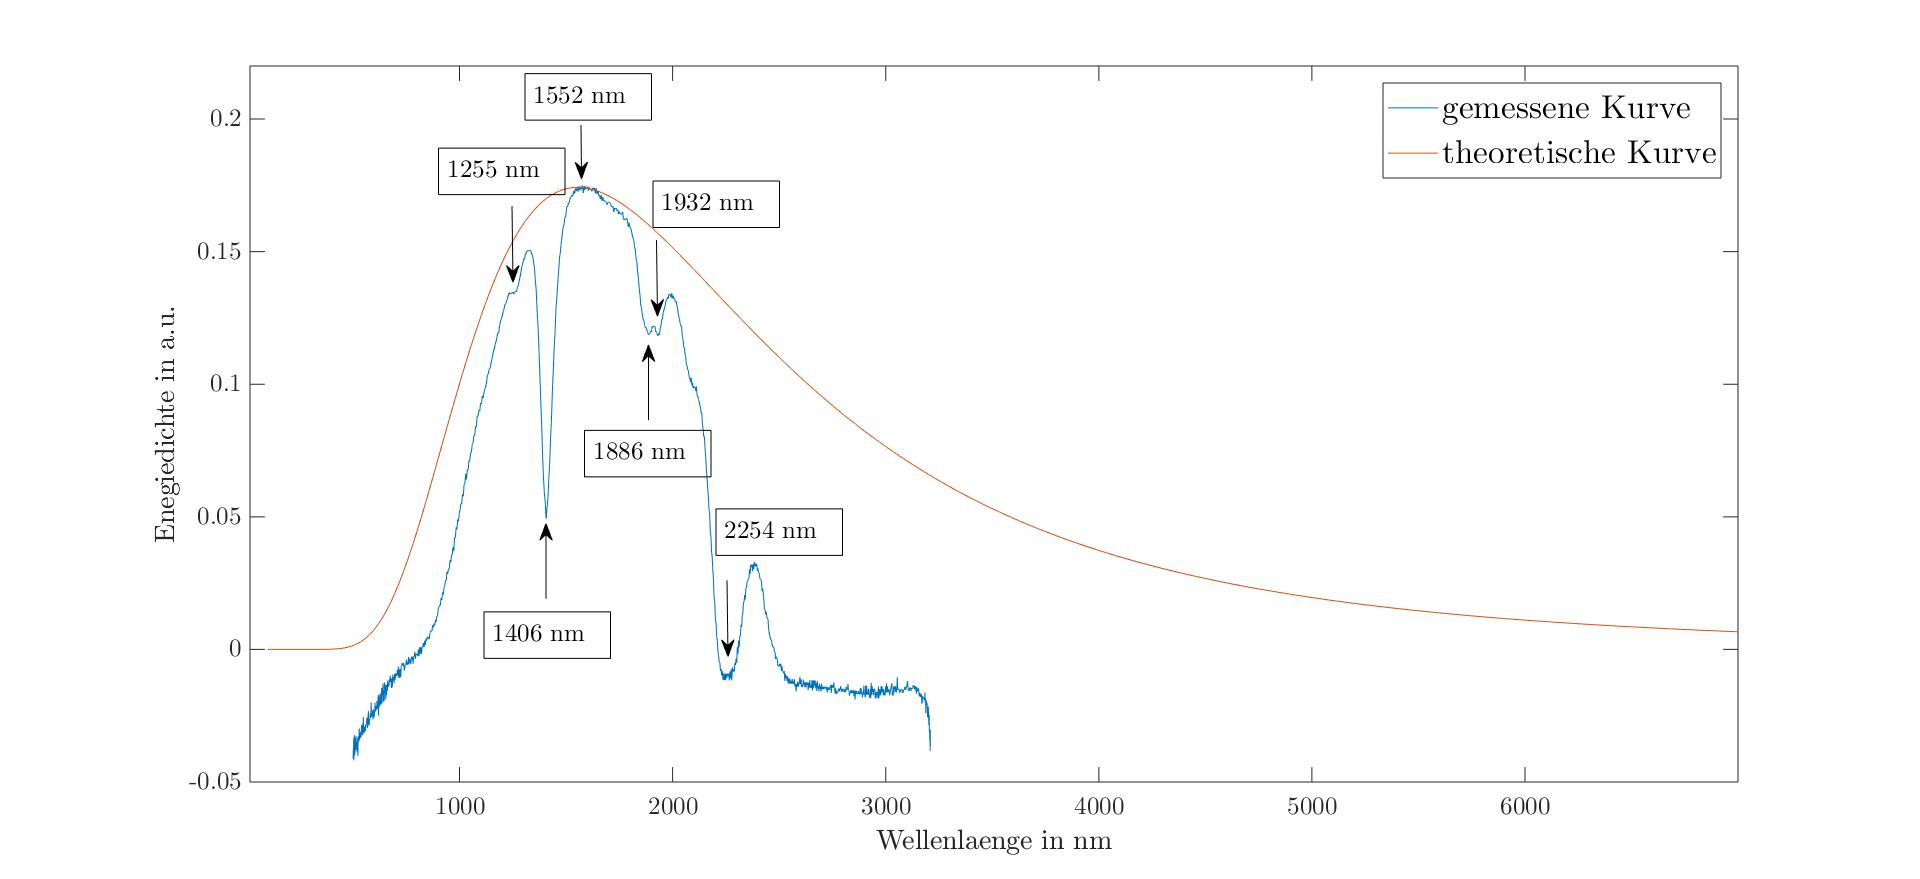
\includegraphics[width=\textwidth]{Bilder/Wolframlampe2V.jpg}
%     \caption{Betriebsspannung = \SI{2}{\volt}}
%   \end{subfigure}
%   \begin{subfigure}{0.9\textwidth}
%     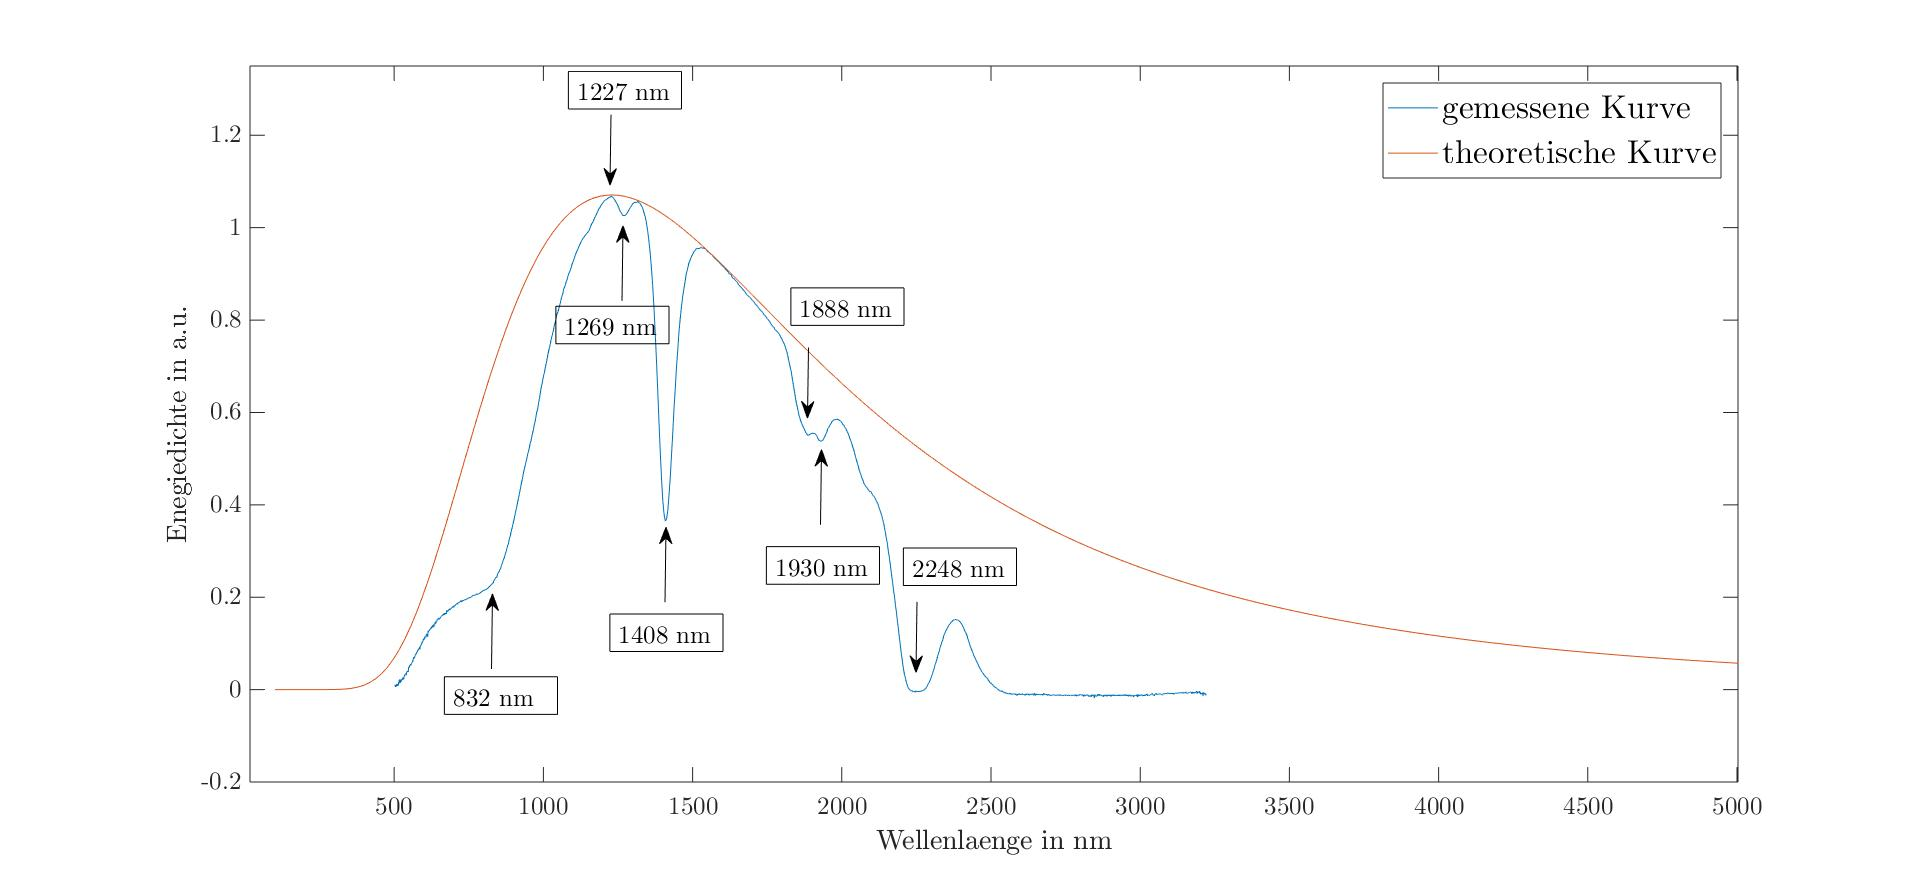
\includegraphics[width=\textwidth]{Bilder/Wolframlampe5V.jpg}
%     \caption{Betriebsspannung = \SI{5}{\volt}}
%   \end{subfigure}\hspace{0.5cm}
%   \caption{spektrale Energiedichte einer Wolframdampflampe bei unterschiedlichen Betriebsspannungen}
%   \label{fig:Wolframlampe}
% \end{figure}
